\section{Challenges}
\label{sec:challenges}

As already stated above in the introduction, nearly every web project bears challenges to solve, both for developers on the one hand, and for content creators on the other hand. While content creators mostly need to solve structural issues in the published content, developers are mainly responsible for supporting authors in technical questions, as well as constantly keeping an eye on the backend development. This might go from always keeping the underlying modules updated, to populating the source code with design or template changes, to finally maintaining the build pipeline and deployment setup.

\subsection{Distributed development}
\label{sec:challenges-distributeddevelopment}

When it comes to administer a static site project, it is very likely, that there will not be any possiblity of working on the same project in the same environment in a linear way. Instead, every developer will have to have a local install of the used generator at his/her disposal, together with access to a remote repository of a version control system for exchanging the current development process with other project maintainers. The main reason for that is the fact, that unlike content authors, developers do have the obligation of installing or maintaining the project's dependencies \cite[85]{dhillon2016}, thus not only for testing reasons.

If using GitHub for example, content editors, on the other hand, may easily make use of the built-in ``In-Page Code Editor'' (see Fig. \ref{fig:github-page-editor} on p. \pageref{fig:github-page-editor}), which also provides an optimistically rendered version of the current content, although without making use of the project's style sheet.

%% Graphic of separating project repositories
\begin{figure} % h-ere, t-op, b-ottom, p-age
    \centering
    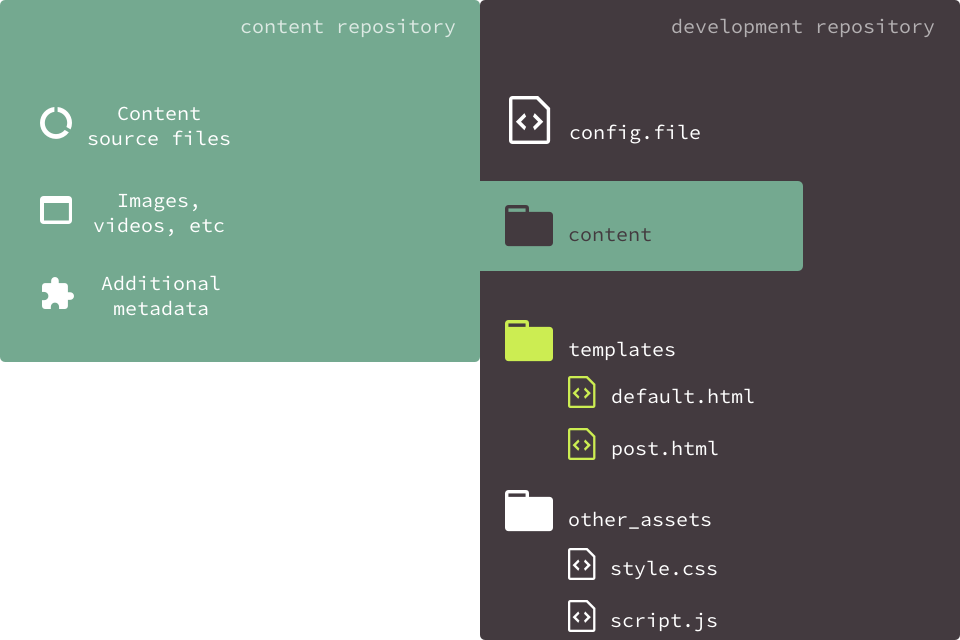
\includegraphics[width=0.9\textwidth]{challenges-repositories.png}
    \caption{A graphic showing the stylized separation of a project into a \emph{content} and a \emph{development} repository. The content authors may only be granted access to the content repository, while developers should be granted access to both, thus providing a seamless integration for the content into the build pipeline flow (see Fig. \ref{fig:build-pipeline} on p. \pageref{fig:build-pipeline}).}
    \label{fig:repository-separation}
\end{figure}
%

\subsubsection{Separating content from code}
As constantly growing static site projects may sooner or later come to a point, where content progression differs from development progression, it might be useful to separate both parts into independent repositories (see Fig. \ref{fig:repository-separation}).


\subsection{Time span for visual feedback}
\label{sec:challenges-timespan}

One of these major challenges remains the issue of providing a ``real website look and feel'' to the content editor. Whereas authors are presented with an already pre-rendered version of the newly added content in dynamic CMSs (since the underlying system is not dependent on any template rendering before deployment), static site generators first offer a glance of the author's work, after the whole build pipeline process succeeded in its render flow.
